\let\negmedspace\undefined
\let\negthickspace\undefined
\documentclass[journal]{IEEEtran}
\usepackage[a5paper, margin=10mm, onecolumn]{geometry}
\usepackage{lmodern} % Ensure lmodern is loaded for pdflatex
\usepackage{tfrupee} % Include tfrupee package

\setlength{\headheight}{1cm} % Set the height of the header box
\setlength{\headsep}{0mm}     % Set the distance between the header box and the top of the text

\usepackage{gvv-book}
\usepackage{gvv}
\usepackage{cite}
\usepackage{amsmath,amssymb,amsfonts,amsthm}
\usepackage{algorithmic}
\usepackage{graphicx}
\usepackage{textcomp}
\usepackage{xcolor}
\usepackage{txfonts}
\usepackage{listings}
\usepackage{enumitem}
\usepackage{mathtools}
\usepackage{gensymb}
\usepackage{comment}
\usepackage[breaklinks=true]{hyperref}
\usepackage{tkz-euclide} 
\usepackage{listings}
\usepackage{gvv}                                       
\def\inputGnumericTable{}                                 
\usepackage[latin1]{inputenc}                                
\usepackage{color}                                            
\usepackage{array}                                            
\usepackage{longtable}                                       
\usepackage{calc}                                             
\usepackage{multirow}                                         
\usepackage{hhline}                                           
\usepackage{ifthen}                                           
\usepackage{lscape}
\usepackage{tikz}
\begin{document}

\bibliographystyle{IEEEtran}
\vspace{3cm}

\title{2008 CE 52-68}
\author{AI24BTECH11019-KOTHA PRATHEEK REDDY}

 \maketitle
%\newpage
% \bigskip
{\let\newpage\relax\maketitle}

\renewcommand{\thefigure}{\theenumi}
\renewcommand{\thetable}{\theenumi}
\setlength{\intextsep}{10pt} % Space between text and floats


\numberwithin{equation}{enumi}
\numberwithin{figure}{enumi}
\renewcommand{\thetable}{\theenumi}
\begin{enumerate}
%q1
	\item A uniform disk of mass $1kg$ and radius $0.1m$ is kept on a surface as shown in the figure. A spring of stiffness $k_1 = 400N/m$ is connected to the disk center $A$ and another spring of stiffness $k_2 = 100N/m$ is connected at point $B$ just above point $A$ on the circumference of the disk. For small disturbance from the equilibruim, the natural frequency of vibration of the system is \underline{\hspace{2cm}} $rad/s$(round off to one decimal place).
		\begin{center}

\resizebox{0.5\textwidth}{!}{%
	\begin{tikzpicture}
    \draw (0,8)--(0,0)--(8,0)--(8,8);
    \draw (0,3)--(1,3)--(1.25,3.5)--(1.5,3)--(1.75,2.5)--(2,3)--(2.25,3.5)--(2.5,3)--(2.75,2.5)--(3,3)--(3.25,3.5)--(3.5,3)--(3.75,2.5)--(4,3);
    \draw (4,3) circle[radius = 3cm];
    \draw (4,3) circle[radius = 0.1cm];
    \draw (4,6) circle[radius = 0.1cm];
    \draw (4,6)--(4.25,6.5)--(4.5,6)--(4.75,5.5)--(5,6)--(5.25,6.5)--(5.5,6)--(5.75,5.5)--(6,6)--(6.25,6.5)--(6.5,6)--(6.75,5.5)--(7,6)--(8,6);
    \node[align = center] at (4.3,2.7){\large $\mathbf{A}$};
    \node[align = center] at (3.7,6.3){\large $\mathbf{B}$};
    \node[align = center] at (2.5,2.3){\large $\mathbf{k_1}$};
    \node[align = center] at (5.5,5.3){\large $\mathbf{k_2}$};
    \draw (-0.5,8)--(0,7);
    \draw (-0.5,7)--(0,6);
    \draw (-0.5,6)--(0,5);
    \draw (-0.5,5)--(0,4);
    \draw (-0.5,4)--(0,3);
    \draw (-0.5,3)--(0,2);
    \draw (-0.5,2)--(0,1);
    \draw (-0.5,1)--(0,0);
    
    \draw (0,0)--(0.5,-0.5);
    \draw (1,0)--(1.5,-0.5);
    \draw (2,0)--(2.5,-0.5);
    \draw (3,0)--(3.5,-0.5);
    \draw (4,0)--(4.5,-0.5);
    \draw (5,0)--(5.5,-0.5);
    \draw (6,0)--(6.5,-0.5);
    \draw (7,0)--(7.5,-0.5);
    \draw (8,0)--(8.5,-0.5);

    
    \draw (8,1)--(8.5,0);
    \draw (8,2)--(8.5,1);
    \draw (8,3)--(8.5,2);
    \draw (8,4)--(8.5,3);
    \draw (8,5)--(8.5,4);
    \draw (8,6)--(8.5,5);
    \draw (8,7)--(8.5,6);
    \draw (8,8)--(8.5,7);
\end{tikzpicture}
}
\end{center} \hfill{[Gate 2019]}
		%q2
	\item A single block brake with a short shoe torque capacity of $250 N.m$ is shown. The cylindrical brake drum rotates anticlockwise at $100rpm$ and the coefficient of friction is $0.25$. The value of $a$, in $mm$(round off to one decimal place), such that the maximum actuating force $P$ is $2000N$, is \underline{\hspace{2cm}}
	
		\begin{center}
	\resizebox{0.5\textwidth}{!}{%
	\begin{tikzpicture}
    \draw (0,0) circle[radius = 5cm];
    \draw[dotted] (-5,0)--(5,0);
    \draw[dotted] (0,5)--(0,-5);
    \draw (-0.25,0.5) -- (-0.25,-0.5) -- (0.25,-0.5) -- (0.25,0.5);
    \draw[thick] (0.25,0.5) arc[start angle=0, end angle=180, radius=0.25cm];
    \draw (-0.25,-0.5)--(0,-0.75);
    \draw (0,-0.5)--(0.25,-0.75);
    \draw (0.25,-0.5)--(0.5,-0.75);
    \draw (0,0) circle[radius = 0.1cm];
    \draw[->] (0,0)--(3,-4);
    \node at (2,-2.5){\large $\mathbf{a}$};
    \draw (-0.2,5)--(0.2,5)--(0.2,5.2)--(-0.2,5.2)--(-0.2,5);
    \draw[thick] (-7.5,5.2) -- (6,5.2);
    \draw (4.8,5.2) -- (4.8,5.8) -- (5.2,5.8) -- (5.2,5.2);
    \draw[thick] (5.2,5.2) arc[start angle=0, end angle=-180, radius=0.2cm];
    \draw (5,5.2) circle[radius = 0.1cm];
    \draw (4.8,5.8)--(5,6);
    \draw (5,5.8)--(5.2,6);
    \draw (5.2,5.8)--(5.4,6);
    \draw (0,5.2) -- (0,8.2);
    \draw[thick,->] (-7.5,8.2)--(-7.5,5.2);
    \draw (5,8.2)--(5,5.2);
    \draw [<->] (-7.5,7.8)--(0,7.8);
    \draw[<->] (0,7.8)--(5,7.8);
    \draw[->](6,5.8)--(6,5.2);
    \draw[->](6,4.4)--(6,5);
    \draw (0,5) -- (6,5);
    \node at (-7.7,7.6){\Large $\mathbf{P}$};
    \node at (-3.25,8){\Large $\mathbf{1.5a}$};
    \node at (2.5,8){\Large $\mathbf{a}$};
    \node at (6.5,5.1){\Large $\mathbf{a/4}$};
\end{tikzpicture}
}
		\end{center}\hfill{[Gate 2019]}
	

%q3
	\item Two immiscible, incompressible, viscous fluids having same densities but different viscosities are contained between two infinite horizontal prallel plates, $2m$ apart as shown below. The bottom plate is fixed and the upper plate moves to the right with a constant velocity of $3m/s$. With the assumptions of Newtonian fluid, steady, and fully developed laminar flow with zero pressure gradient in all directions, the momentum equations simplify to
		\begin{align}
			\frac{d^2u}{dy^2} &= 0;
		\end{align}
If the dynamic viscosity of the lower fluid, $\mu_2$, is twice that of the upper fluid,$\mu_1$, then the velocity at the interface (round off to two decimal places) is \underline{\hspace{2cm}}$m/s$.
\begin{center}

\resizebox{0.8\textwidth}{!}{%
 \begin{tikzpicture}
    \draw[->] (-5,0)--(-2,0);
    \draw[->] (-5,0)--(-5,3);
    \node at (-2.5,-0.25){\large $\mathbf{x}$};
    \node at (-5.25,2.5){\large $\mathbf{y}$};
    \draw (0,0) -- (6,0);
    \draw (0,3) -- (6,3);
    \draw (0,1.5) -- (6,1.5);
    \draw (0,1.5)--(1,3);
    \draw (1,1.5)--(2,3);
    \draw (2,1.5)--(3,3);
    \draw (3,1.5)--(4,3);
    \draw (4,1.5)--(5,3);
    \draw (5,1.5)--(6,3);
    \draw (0,1.5)--(1,0);
    \draw (1,1.5)--(2,0);
    \draw (2,1.5)--(3,0);
    \draw (3,1.5)--(4,0);
    \draw (4,1.5)--(5,0);
    \draw (5,1.5)--(6,0);
    \node[align = center] at (3,2){\large $\mathbf{\mu _1}$};
     \node[align = center] at (3,1){\large $\mathbf{\mu _2}$};
     \draw[<->] (-0.5,0)--(-0.5,3); 
     \node[align=center] at (-0.8,1.5){$\mathbf{2m}$};
     \draw[->] (3,3.2)--(6,3.2);
     \draw[<->] (6.5,1.5)--(6.5,0); 
     \node[align=center] at (6.8,0.75){$\mathbf{1m}$};
     \node at (8,1.5){\large $\mathbf{\mu _2 = 2\mu _1}$};
     
\end{tikzpicture}
}
\end{center}\hfill{[Gate 2019]}
%q4
	\item A cube of side $100mm$ is placed at the bottom of an empty container on one of its faces. The density of the material of the cube is $800kg/{m^3}$. Liquid of density $1000 kg/{m^3}$ is now poured into the container. The minimum height to which the liquid needs to be poured into the container for the cube to just lift up is \underline{\hspace{2cm}}$mm$. \hfill{[Gate 2019]}
%q5
	\item Three slabs are joined together as shown in the figure. There is no thermal contact resistance at the interfaces. The center slab experiences a non-uniform internal heat generation with an average value to $10000 Wm^{-3}$, while the left and right slabs have no internal heat generation. All slabs have thickness equal to $1m$ and thermal conductivity of each slab is equal to$5Wm^{-1}K^{-1}$. The two extreme faces are exposed to fluid with heat transfer coefficient $100Wm^{-2}K^{-1}$ and bulk temperature $30^{\circ}C$ as shown. The heat transfer in the slabs is assumed to be one dimesional and steady, and all properties are constant. If the left extreme face temperature $T_1$ is measured to be $100^{\circ}C$, the right extreme face temperature $T_2$ is \underline{\hspace{2cm}}$^{\circ}C$.
		\begin{figure}[h]
\centering
\resizebox{0.5\textwidth}{!}{%
	\begin{tikzpicture}
    \draw (0,-4)--(0,4);
    \draw (2,-4)--(2,4);
    \draw (4,-4)--(4,4);
    \draw (6,-4)--(6,4);
    \node[align=center] at (-1.3,2){Left extreme \\face $T_1 =100^{\circ}$C};
    \node[align = center] at (-1.3,-2){$100 W/{m^2}.K$\\$30^{\circ}C$};
    \draw[->] (-1.3,-4) -- (-1.3,-2.5);
     \node[align = center] at (7.3,-2){$100 W/{m^2}.K$\\$30^{\circ}C$};
    \draw[->] (7.3,-4) -- (7.3,-2.5);
    \draw[<->] (0,2)--(2,2);
    \draw[<->] (2,2)--(4,2);
    \draw[<->] (4,2)--(6,2);
    \node at (1,1.5){$1m$};
    \node at (3,1.5){$1m$};
    \node at (5,1.5){$1m$};
    \node at (6.5,2){$T_2$};
    
\end{tikzpicture}
}
\end{figure}\hfill{[Gate 2019]}
%q6
	\item If one mole of $H_2$ gas occupies a rigid container with a capacity of $1000$ litres and the temperature is raised from $27^{\circ}C$ to $37^{\circ}C$, the change in pressure of the contained gas(round off to two decimal places), assuming ideal gas behaviour, is \underline{\hspace{2cm}}$Pa.$\brak{R = 8.314 J/{mol.K} 	}\hfill{[Gate 2019]}
%q7
	\item A steam power cycle with regeneration as shown below on the $T-s$ diagram employs a single open feedwater heater for efficiency improvement. The fluids mix with each other in an open feedwater heater. The turbine is isentropic and the input(bleed) to the feedwater heater from the turbine is at state 2 as shown in the figure. Process 3-4 occurs in the condenser. The pump work is negligible. The input to the boiler at state 5. The follwoing information is available from the stream tables:
	\begin{table}[h]
		\centering
	\begin{tabular}{|c|c|c|c|c|c|c|}
		\hline
		State & 1&2&3&4&5&6\\
		\hline
		Enthalpy\brak{kJ/kg}&3350&2800&2300&175&700&1000\\
		\hline
	\end{tabular}
	\end{table}
	<\begin{figure}[h]
%\centering
%\resizebox{0.8\textwidth}{!}
\end{figure} 
The mass flow rate of steam bled from the turbine as a percentage of the total mass flow rate at the inlet to the turbine at state 1 is \underline{\hspace{2cm}}\hfill{[Gate 2019]}
%q8
	\item A gas turbine with air as the working fluid has an isentropic efficiency of $0.70$ when operating at a pressure ratio of $3$. Now the pressure ratio of the turbine is increased to 5, while maintaining the same inlet conditions. Assume air as a perfect gas with specific heat ratio $\gamma = 1.4$. If the specific work output remains the same for both the cases, the isentropic efficiency of the turbine at the pressure ratio of 5 is \underline{\hspace{2cm}}(round off to two decimal places)\hfill{[Gate 2019]}
%q9
	\item The value of the following definite integral is \underline{\hspace{2cm}}(round off to two decimal places)
	\begin{align}
	\int_1^e \brak{x\ln{x}}dx \notag
	\end{align}\hfill{[Gate 2019]}
%q10
	\item In ASA system, the side cutting and end cutting edge angles of a sharp turning tools are $45^{\circ}$ and $10^{\circ}$, respectively. The feed during cylindrical turning is $0.1mm/{rev}$. The center line average surface roughness(in $\mu m$, round off to one decimal place) of the generated surface is \underline{\hspace{2cm}}.\hfill{[Gate 2019]}
%q11
	\item Taylor's tool life equation is given by $VT^n = C$, where $V$ is in $m/{min}$ and $T$ is in $min$. In a turning operation, two tools $X$ and $Y$ are used. For tool $X$, $n = 0.3$ and $C=60$ and for tool $Y$, $n=0.6$ and $C=90$. Both the tools will have the same tool life for the cutting speed(in $m/min$, round off to one decimal place) of \underline{\hspace{2cm}}\hfill{[Gate 2019]}
%q12
	\item Five jobs \brak{J1,J2,J3,J4,J5} need to be processed in a factory. Each job can be assigned to any of the five different machines \brak{M1,M2,M3,M4,M5}. The time durations taken(in minutes) by machines for each of the jobs, are given in the table. However each job is assigned to a specific machine in such a way that the total processing time is minimum. The total processing time is \underline{\hspace{2cm}} minutes.
		\begin{table}[h]
		\centering
	\begin{tabular}{|c|c|c|c|c|c|}
	\hline
	&$M1$&$M2$&$M3$&$M4$&$M5$\\
	\hline
	$J1$&40&30&50&50&58\\
	\hline
	$J2$&26&38&60&26&38\\
	\hline
	$J3$&40&34&28&24&30\\
	\hline
	$J4$&28&40&40&32&48\\
	\hline
	$J5$&28&32&38&22&44\\
	\hline
	\end{tabular}
	\end{table}\hfill{[Gate 2019]}
%q13
	\item A project consists of six activities. The immidiate predeccesor of each acticity and the estimated duration is also provided in the table below:\\
		\begin{table}[h]
			\centering
	\begin{tabular}{|c|c|c|}
	\hline
		Activity&Immediate predecessor&Estimated duration(weeks)\\
		\hline
		$P$&-&5\\
		\hline
		$Q$&-&1\\
		\hline
		$R$&$Q$&2\\
		\hline
		$S$&$P,R$&4\\
		\hline
		$T$&$P$&6\\
		\hline
		$U$&$S,T$&3\\
		\hline
	\end{tabular}
		\end{table}
	If all acticities other than $S$ take the estimated amount of time, the maximum duration(in weeks) of the activity S without delaying the completion of the project is \underline{\hspace{2cm}}\hfill{[Gate 2019]}



\end{enumerate}
\end{document}
